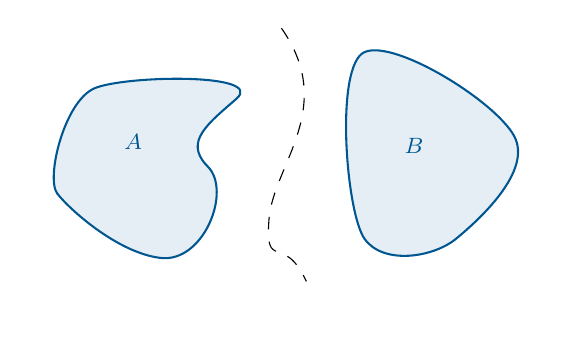
\begin{tikzpicture}[x=0.75pt,y=0.75pt,yscale=-1,xscale=1]
	%uncomment if require: \path (0,300); %set diagram left start at 0, and has height of 300

	%Shape: Polygon Curved [id:ds20022184980649105] 
	\draw  [color={rgb, 255:red, 0; green, 86; blue, 145 }  ,draw opacity=1 ][fill={rgb, 255:red, 0; green, 86; blue, 145 }  ,fill opacity=0.1 ][line width=0.75]  (47.85,39.3) .. controls (62.33,33.02) and (130.77,31.76) .. (116.3,44.33) .. controls (102.26,56.52) and (91.54,64.77) .. (101.55,75.96) .. controls (101.86,76.31) and (102.19,76.66) .. (102.54,77.01) .. controls (114.2,88.74) and (100.53,123.52) .. (79.7,121) .. controls (58.88,118.49) and (35.66,97.37) .. (30,90) .. controls (24.34,82.63) and (33.38,45.59) .. (47.85,39.3) -- cycle ;
	%Shape: Polygon Curved [id:ds5640401880667114] 
	\draw  [color={rgb, 255:red, 0; green, 86; blue, 145 }  ,draw opacity=1 ][fill={rgb, 255:red, 0; green, 86; blue, 145 }  ,fill opacity=0.1 ][line width=0.75]  (178.05,21.82) .. controls (192.52,15.53) and (240.75,45.29) .. (250.05,62.15) .. controls (259.34,79.02) and (233.05,102.82) .. (222.05,111.82) .. controls (211.05,120.82) and (187.05,124.48) .. (178.05,111.82) .. controls (169.05,99.15) and (163.57,28.1) .. (178.05,21.82) -- cycle ;
	%Curve Lines [id:da7601976291136298] 
	\draw  [dash pattern={on 4.5pt off 4.5pt}]  (138,10.33) .. controls (165,48.67) and (134,76.33) .. (132,102.33) .. controls (130,128.33) and (139,108.33) .. (150,132.33) ;

	% Text Node
	\draw (61,60) node [anchor=north west][inner sep=0.75pt]  [font=\footnotesize,color={rgb, 255:red, 0; green, 86; blue, 145 }  ,opacity=1 ]  {$A$};
	% Text Node
	\draw (196.05,62.02) node [anchor=north west][inner sep=0.75pt]  [font=\footnotesize,color={rgb, 255:red, 0; green, 86; blue, 145 }  ,opacity=1 ]  {$B$};
	% Text Node
	\draw (16,150) node [anchor=north west][inner sep=0.75pt]   [align=left] {};


\end{tikzpicture}
